% This is the Reed College LaTeX thesis template. Most of the work 
% for the document class was done by Sam Noble (SN), as well as this
% template. Later comments etc. by Ben Salzberg (BTS). Additional
% restructuring and APA support by Jess Youngberg (JY).
% Your comments and suggestions are more than welcome; please email
% them to cus@reed.edu
%
% See http://web.reed.edu/cis/help/latex.html for help. There are a 
% great bunch of help pages there, with notes on
% getting started, bibtex, etc. Go there and read it if you're not
% already familiar with LaTeX.
%
% Any line that starts with a percent symbol is a comment. 
% They won't show up in the document, and are useful for notes 
% to yourself and explaining commands. 
% Commenting also removes a line from the document; 
% very handy for troubleshooting problems. -BTS

% As far as I know, this follows the requirements laid out in 
% the 2002-2003 Senior Handbook. Ask a librarian to check the 
% document before binding. -SN

%%
%% Preamble
%%
% \documentclass{<something>} must begin each LaTeX document
\providecommand{\main}{.}
\documentclass[12pt,twoside]{reedthesis}
% Packages are extensions to the basic LaTeX functions. Whatever you
% want to typeset, there is probably a package out there for it.
% Chemistry (chemtex), screenplays, you name it.
% Check out CTAN to see: http://www.ctan.org/
%%
\usepackage{graphicx,latexsym} 
\usepackage{amssymb,amsthm,amsmath}
\usepackage{longtable,booktabs,setspace} 
\usepackage{chemarr} %% Useful for one reaction arrow, useless if you're not a chem major
\usepackage[hyphens]{url}
\usepackage{rotating}
\usepackage{hyperref}

\usepackage{physics}
\usepackage{siunitx}
\usepackage[subpreambles]{standalone}
% \usepackage{natbib}
% Comment out the natbib line above and uncomment the following two lines to use the new 
% biblatex-chicago style, for Chicago A. Also make some changes at the end where the 
% bibliography is included. 
%\usepackage{biblatex-chicago}
%\bibliography{thesis}

% \usepackage{times} % other fonts are available like times, bookman, charter, palatino

\title{TITLE TBD}
\author{Kees Benkendorfer}
% The month and year that you submit your FINAL draft TO THE LIBRARY (May or December)
\date{May 2021}
\division{Mathematics and Natural Sciences}
\advisor{Andrew Larkoski}
%If you have two advisors for some reason, you can use the following
%\altadvisor{Your Other Advisor}
%%% Remember to use the correct department!
\department{Physics}
% if you're writing a thesis in an interdisciplinary major,
% uncomment the line below and change the text as appropriate.
% check the Senior Handbook if unsure.
%\thedivisionof{The Established Interdisciplinary Committee for}
% if you want the approval page to say "Approved for the Committee",
% uncomment the next line
%\approvedforthe{Committee}

\setlength{\parskip}{0pt}

%%
%% End Preamble
%%
%% The fun begins:
\begin{document}

  \maketitle
  \frontmatter % this stuff will be roman-numbered
  \pagestyle{empty} % this removes page numbers from the frontmatter

% Acknowledgements (Acceptable American spelling) are optional
% So are Acknowledgments (proper English spelling)
    \chapter*{Acknowledgements}
	I want to thank a few people.

% The preface is optional
% To remove it, comment it out or delete it.
    \chapter*{Preface}
	This is an example of a thesis setup to use the reed thesis document class.
	
	

    \chapter*{List of Abbreviations}

	\begin{table}[h]
	\centering % You could remove this to move table to the left
	\begin{tabular}{ll}
		\textbf{QCD}  	&  Quantum chromodynamics \\
		\textbf{SCET}  	&  Soft collinear effective theory\\
	\end{tabular}
	\end{table}
	

    \tableofcontents
% if you want a list of tables, optional
    \listoftables
% if you want a list of figures, also optional
    \listoffigures

% The abstract is not required if you're writing a creative thesis (but aren't they all?)
% If your abstract is longer than a page, there may be a formatting issue.
    \chapter*{Abstract}
	The preface pretty much says it all.
	
	\chapter*{Dedication}
	You can have a dedication here if you wish.

  \mainmatter % here the regular arabic numbering starts
  \pagestyle{fancyplain} % turns page numbering back on

%The \introduction command is provided as a convenience.
%if you want special chapter formatting, you'll probably want to avoid using it altogether

\chapter*{Introduction}
     \addcontentsline{toc}{chapter}{Introduction}
\chaptermark{Introduction}
\markboth{Introduction}{Introduction}
% The three lines above are to make sure that the headers are right, that the intro gets included in the table of contents, and that it doesn't get numbered 1 so that chapter one is 1.

	Introduction here

	\section{Technical and notational conventions}

	First, we hold Planck's constant and the speed of light to be equal to unity: $\hbar = c = 1$. It turns out that non-unity values of these quantities are, for our purposes, redundant; when converting a given quantity to SI units, the appropriate factors of $c$ and $\hbar$ can be intuited from context. The result is that all quantities will be measured in units of energy. Physics where we will be working is at the \si{\giga\electronvolt} scale and higher. Therefore, to a high degree of accuracy, we will assume all particles to be massless.

	Unless otherwise stated (and we \textit{will} eventually state otherwise), we will work in $4$ dimensions, comprising the usual three spatial dimensions and one temporal dimension. Vectors in $4$ dimensions (called four-vectors) are denoted by a Greek-letter index and take the form
	\begin{equation}
		p^\mu = (p^0, p^1, p^2, p^3).
	\end{equation}
	The $0$-th component of a four-vector is its `time' (or equivalent) component, and the others are the `spatial' (or equivalent) components. Thus, for example, a four-vector representing position would be
	\begin{equation}
		x^\mu = (t, x, y, z),
	\end{equation}
	while a four-momentum has the components
	\begin{equation}
		p^\mu = (E, p_x, p_y, p_z)
	\end{equation}
	with energy taking the place of time. It is sometimes convenient to refer to lower-dimensional pieces of a four-vector (usually two or three of the spatial components). When doing so, we will denote the sub-vector using a bold-face letter:
	\begin{equation}
		p^\mu = (E, \vb{p}), \quad \vb{p} = (p_x, p_y, p_z).
	\end{equation}

	As is standard in high-energy physics, we will neglect the effects of gravity and assume we are working in a flat space-time. When combining four-vectors, we will therefore use the `mostly minus' metric\footnote{Also known as the `West Coast' metric, among other names. The `East Coast' metric takes the opposite sign convention. Our convention here is clearly the correct one, as it results in naturally positive masses.}
	\begin{equation}
		\eta^{\mu \nu} = \begin{pmatrix}
			1 & 0 & 0 & 0 \\
			0 & -1 & 0 & 0 \\
			0 & 0 & -1 & 0 \\
			0 & 0 & 0 & -1
		\end{pmatrix}.
	\end{equation}
	We will also employ the Einstein summation notation, in which one sums over repeated indices in an expression (known as `contracting' the index). Hence, for $p^\mu = (p^0, \vb{p})$ and $k_\mu = (k_0, \vb{k})$, we have
	\begin{equation}
		k_\mu p^\mu = k_0 p^0 + k_1 p^1 + k_2 p^2 + k_3 p^3.
	\end{equation}

	With our choice of metric, there is little mechanical difference between a contravariant and a covariant four-vector; one picks up a formal minus sign in the spatial components, but that is all. We will, therefore, not distinguish between the two, and we will interchange upper and lower indices freely, bearing in mind that contracting an index negates the spatial terms of the sum. Hence, for $p^\mu = (p^0, \vb{p})$ and $k^\mu = (k^0, \vb{k})$, we will write\footnote{Sorry, Joel.}
	\begin{equation}
		k^\mu p_\mu = k_\mu p^\mu = k^\mu p^\mu = k_\mu p_\mu = k^0 p^0 - \vb{k} \cdot \vb{p}.
	\end{equation}
	The final term is the standard dot product between the three-vectors. This choice enables us to abuse notation in a convenient manner: we will often drop the Greek sub/superscript on four-vectors, and use the standard notation of linear algebra to indicate their contraction:
	\begin{equation}
		k \cdot p = k^0 p^0 - \vb{k}\cdot\vb{p}.
	\end{equation}

	Let us end with a reminder about the connection between these four-vectors and the physical world. Suppose a particle has a momentum four-vector $p^\mu$. Transforming our frame of reference to the particle's rest frame, we could write $p^\mu = (E, 0, 0, 0)$, where $E$ is the particle's energy. But then, recalling the famous relation $E = mc^2 = m$ (since we set $c = 1$), we have
	\begin{equation}
		p^2 = p \cdot p = E^2 = m^2.
	\end{equation}
	Thus, the square of a particle's four-momentum yields its squared mass. Recall now that we are assuming all particles to be massless; therefore, for any `on-shell' particle (that is, a particle that could exist on its own and not just in some quantum fluctuation), we see that $p^2 = 0$, and also that $E^2 = \vb{p} \cdot \vb{p}$.\footnote{This is not strictly an accurate proof of these properties, since massless particles move at the speed of light and one cannot boost into a light-like reference frame using Lorentz transformations. But the spirit of the argument is right, and the result is the same regardless.} This will greatly simplify our calculations later on.

	

\chapter{QCD, jet grooming, and SCET}
	
	First chapter here

	\section{Quantum Chromodynamics (QCD)}

	\section{Jets}

	\section{mMDT Grooming}

	\section{Soft Collinear Effective Theory (SCET)}


\chapter{Leading-order calculation}

	\section{Setup}

	\section{Dimensional regularization}

	\section{Putting it all together}


\chapter{Factorization formula}
	
	\graphicspath{{factorization/figures/}}

	% This is the Reed College LaTeX thesis template. Most of the work 
% for the document class was done by Sam Noble (SN), as well as this
% template. Later comments etc. by Ben Salzberg (BTS). Additional
% restructuring and APA support by Jess Youngberg (JY).
% Your comments and suggestions are more than welcome; please email
% them to cus@reed.edu
%
% See http://web.reed.edu/cis/help/latex.html for help. There are a 
% great bunch of help pages there, with notes on
% getting started, bibtex, etc. Go there and read it if you're not
% already familiar with LaTeX.
%
% Any line that starts with a percent symbol is a comment. 
% They won't show up in the document, and are useful for notes 
% to yourself and explaining commands. 
% Commenting also removes a line from the document; 
% very handy for troubleshooting problems. -BTS

% As far as I know, this follows the requirements laid out in 
% the 2002-2003 Senior Handbook. Ask a librarian to check the 
% document before binding. -SN

%%
%% Preamble
%%
% \documentclass{<something>} must begin each LaTeX document
\providecommand{\main}{..}
\documentclass[12pt,twoside,class=../reedthesis, crop=false]{standalone}
% Packages are extensions to the basic LaTeX functions. Whatever you
% want to typeset, there is probably a package out there for it.
% Chemistry (chemtex), screenplays, you name it.
% Check out CTAN to see: http://www.ctan.org/
%%
\usepackage{graphicx,latexsym} 
\usepackage{amssymb,amsthm,amsmath}
\usepackage{longtable,booktabs,setspace} 
\usepackage{chemarr} %% Useful for one reaction arrow, useless if you're not a chem major
\usepackage[hyphens]{url}
\usepackage{rotating}
\usepackage{hyperref}

\usepackage{physics}
\usepackage{siunitx}
\usepackage{xcolor}
% \usepackage{standalone}
% \usepackage{natbib}
% Comment out the natbib line above and uncomment the following two lines to use the new 
% biblatex-chicago style, for Chicago A. Also make some changes at the end where the 
% bibliography is included. 
%\usepackage{biblatex-chicago}
%\bibliography{thesis}

% \usepackage{times} % other fonts are available like times, bookman, charter, palatino

\newcommand{\zcut}{\mathrm{z_{cut}}}


\setlength{\parskip}{0pt}
%%
%% End Preamble
%%
%% The fun begins:
\begin{document}
	The first step on the path to an all-orders calculation is to derive a factorization formula for the heavy hemisphere mass cross section. The basic process for doing so is laid out in technical detail in Ref.~\cite{becher_introduction_2015-1}, and an example of a similar flavor to our calculation is provided by Frye et al.\ in Ref.~\cite{frye_factorization_2016}.\footnote{Indeed, the calculation of Frye et al.\ is a more general factorization of mass-like variables in groomed jets. Setting $\alpha = 2, \beta = 0$ for their two-point energy correlation function $e_2^{(\alpha)}$ under soft drop grooming with angular exponent $\beta$ yields the mMDT-groomed jet mass $\rho$. Their factorization is valid in the limit $\rho \ll \zcut \ll 1$, whereas we are interested in the limit $\rho \sim \zcut \ll 1$.} There are two primary steps in developing a factorization formula:
	\begin{enumerate}
		\item \textbf{Power counting}: this involves determining the possible radiative modes of an event and their dominant momentum scales. The term `power counting' refers to the fact that for some momentum scale $\lambda$, different radiative modes have momenta that scale as different powers of $\lambda$.

		\item \textbf{Factorization and refactorization}: Once the different radiative modes and energy scales are identified, we can use the framework of SCET to split the cross section into a convolution of terms describing different radiative modes. These terms themselves must then be split (refactored) into convolutions of terms, each of which depends, to leading order, only on a single energy scale.
	\end{enumerate}

\section{Setup}
	Recall that the hemisphere mass is defined to be
	\begin{equation}
		\rho = \frac{1}{E_J^2} \sum_{i<j} 2p_i \cdot p_j
	\end{equation}
	with $E_J$ the jet energy and the sum ranging over all pairs of particles in the jet. Expanding out the dot product, we have
	\begin{equation}\label{eq:jet mass z theta}
		\rho = \frac{2}{E_J^2} \sum_{i<j} \qty(E_i E_j - \vb{p}_i \cdot \vb{p}_j) = \frac{2}{E_J^2} \sum_{i<j} E_i E_j \qty(1 - \cos\theta_{ij}) = \sum_{i<j}2z_i z_j \qty(1 - \cos\theta_{ij}).
	\end{equation}
	Here, $z_i$ and $z_j$ are the relative energy fractions of each particle and $\theta_{ij}$ is the angle between particles $i$ and $j$.

	Throughout the following discussion, with $n^\mu$ the jet direction and $\bar n^\mu$ the direction opposite the jet, we will describe momenta in light-cone coordinates
	\begin{equation}
		p^\mu = \qty(p^-, p^+, p_\perp)
	\end{equation}
	with
	\begin{align}
		p^- &= \bar n \cdot p & p^+ &= n \cdot p
	\end{align}
	and $p_\perp$ the components of momentum transverse to $n$. In these coordinates, the energy fraction with respect to total energy $E_J = Q$ is
	\begin{equation}\label{eq:z light cone coordinates}
		z = \frac{p^+ + p^-}{2Q}
	\end{equation}
	and, in the collinear limit, the angle to the jet axis is $\theta \approx p_\perp / p^0$ \cite{frye_factorization_2016}.
	
	In an $e^+ e^- \to \text{jets}$ event, there are two types of emission: resolved and unresolved. The essential difference is that a resolved emission is one which manifests itself as a jet at a particular scale of observation, while an unresolved emission does not. The presence of unresolved emissions can, however, perturb observable values of a resolved emission. {\color{red}\textbf{[TODO: check that this is a reasonable description]}} 

	Suppose now that we have applied an mMDT groomer with energy fraction cutoff $\zcut$. Then every \textit{resolved} emission must satisfy
	\begin{equation}
		z_i > \zcut,
	\end{equation}
	while other emissions with $z_i < \zcut$ can only pass the groomer if they are at a sufficiently small angle to a resolved emission.

\section{Power counting}
\subsection{Resolved soft emission}
	The primary emission contributing to the jet mass in the limit $\rho \sim \zcut \ll 1$ is a gluon emission $z_i$ sensitive to both $\rho$ and $\zcut$. In the presence of a hard quark (i.e., the jet) with $z_q \sim 1$, leading contributions to the jet mass of Eq.~\ref{eq:jet mass z theta} is
	\begin{equation}
		\rho \approx \sum_i 2z_i \qty(1 - \cos\theta_i)
	\end{equation}
	where $\theta_i$ is the angle of emission $i$ from the quark. Considering the case with only one such emission,\footnote{This is the one-loop contribution {\color{red}\textbf{[is this accurate?]}}.} we have
	\begin{equation}
		\rho \approx z_i \qty(1 - \cos\theta_i).
	\end{equation} 
	But since $z_i \sim \zcut$ and $\rho \sim \zcut$, this means that
	\begin{equation}
		\rho \approx \rho \qty(1 - \cos\theta_i),
	\end{equation}
	so
	\begin{equation}
		\cos\theta_i \ll 1.
	\end{equation}
	This means that
	\begin{equation}
		\theta_i \sim \frac{\pi}{2}.
	\end{equation}
	Since this emission is sensitive to $\zcut \ll 1$, we can also conclude that $z_i \ll 1$. Thus, we see that the leading contribution to the cusp region comes from a \textbf{resolved soft, wide-angle} gluon. Its momentum scales like
	\begin{equation}
		p_R \sim \zcut Q \qty(1, 1, 1).
	\end{equation}
	For future reference, let this gluon have energy fraction $z_R$ and angle $\theta_R$ from the quark axis.

\subsection{Ungroomed extra-soft unresolved radiation}
	\begin{figure}
	\begin{centering}
		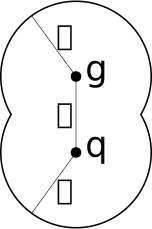
\includegraphics[width=0.2\columnwidth]{\main/factorization/figures/head_on_schematic.pdf}
		\caption{\label{fig:head-on schematic}Head-on schematic of a quark jet $q$ and a resolved gluon $g$. If the angle between the quark and the gluon is $\theta$ and the gluon (plus all lower-scale unresolved radiation) passes the groomer, then the mMDT groomer will accept all radiation within an angle $\theta$ of both the quark and the resolved gluon.}
	\end{centering}
	\end{figure}
	Unresolved soft emissions can also contribute to the jet mass if they are sufficiently close to the resolved emission or the quark. Suppose there is another emission $i$ with energy fraction $z_i$ at angle $\theta_i$ from the jet axis and angle $\theta_{iR}$ from the resolved gluon. If $\theta_i < \theta_R$ or $\theta_iR < \theta_R$, a situation displayed in Fig.~\ref{fig:head-on schematic}, then emission $i$ will pass the groomer.

	What does this mean for the hemisphere mass? Well, first notice that since $\theta_R \sim \pi/2$, most soft radiation in the hemisphere passes this cut. The effect of these extra-soft emissions, which have $z_i \ll z_R$, is to perturb the mass of the resolved emission, so that the hemisphere mass is approximately
	\begin{equation}
		\rho \sim z_R + \sum_i z_i(1 - \cos\theta_i).
	\end{equation}
	The dominant contributions come again from the wide-angle emissions with $1 - \cos\theta_i \sim 1$; these must evidently have an energy scale set by
	\begin{equation}
		\rho - z_R \sim \sum_i z_i.
	\end{equation}
	Hence, since $z_R \sim \zcut$, the unresolved extra-soft emissions must scale as
	\begin{equation}
		p_{S_R} \sim \qty(\rho - \zcut)Q(1, 1, 1).
	\end{equation}

\subsection{Groomed soft radiation}
	Radiation outside of the region displayed in Fig.~\ref{fig:head-on schematic} gets groomed away if its energy fraction is
	\begin{equation}
		z_i < \zcut.
	\end{equation}
	If $z_i > \zcut$, then we would have a second resolved emission, which we have already decided to ignore. These emissions must be at a very wide angle in order to not be within the region of mMDT acceptance. Since this \textbf{global soft} radiation is removed by the groomer, it is not sensitive to $\rho$ and contributes only to the normalization. It must scale as
	\begin{equation}
		p_{S_G} \sim \zcut Q(1, 1, 1).
	\end{equation}

\subsection{Collinear radiation}\label{sec:collinear radiation}
	Finally, we consider radiation collinear to a jet axis with angle $\theta_i \ll 1$. This radiation has $p^- \gg p^+$, which means from Eq.~\ref{eq:z light cone coordinates} that
	\begin{equation}
		z \approx \frac{p^+}{2Q}.
	\end{equation}
	Then because the particle must satisfy
	\begin{equation}
		z_i \theta_i^2 \lesssim \rho,
	\end{equation}
	we find that \cite{frye_factorization_2016}
	\begin{equation}
		\rho \sim \frac{p^+}{Q}.
	\end{equation}

	If $z \sim 1$, we know that $z \gg \zcut$, so the momentum scales independently of $\zcut$. Hence, the scaling of these \textbf{collinear} modes is \cite{frye_factorization_2016}
	\begin{equation}
		p_c \sim Q \qty(1, \rho, \rho^{1/2}).
	\end{equation}
	In a hemisphere where the resolved emission stops the mMDT groomer, this is the only collinear radiation that contributes {\color{red}\textbf{[TODO: ask Andrew: is this correct?]}}.

	If on the other hand $z \sim \zcut \ll 1$, the result is \textbf{collinear-soft} radiation with $p^- \sim z_i Q$ and $p^+ \sim \theta_i^2 z_i Q$. From \cite{frye_factorization_2016}, these momenta scale like
	\begin{equation}
		p_{cs} \sim \zcut Q \qty(1, \frac{\rho}{\zcut}, \qty(\frac{\rho}{\zcut})^{1/2})
	\end{equation}
	and depend on the single energy scale $\sqrt{\rho\,\zcut}$. This scale matters in the hemisphere which does not contain the resolved soft gluon.


\section{Factorization}
	With the power counting in hand, we are now ready to derive a factorization formula describing the hemisphere mass distribution in the limit $\rho \sim \zcut \ll 1$. First, we should note that it is most straightforward to compute the double differential cross section in the masses of the individual hemispheres, then integrate over them to get the heavy hemisphere mass \cite{chien_resummation_2010}:
	\begin{equation}\label{eq:heavy hemisphere cross section}
		\frac{d\sigma}{d\rho} = \int \frac{d^2\sigma}{d\rho_1d\rho_2}\qty[\delta(\rho - \rho_1)\Theta(\rho_1 - \rho_2) + \delta(\rho - \rho_2)\Theta(\rho_2 - \rho_1)].
	\end{equation}
	The integral simply breaks up the two cases $\rho_1 > \rho_2$ and $\rho_2 > \rho_1$ and assigns the correct value of $\rho$ in each case.

	Now, in the limit $\rho_1, \rho_2 \ll 1$, we can apply the technology of SCET to factorize the double-differential cross section into a product of hard, soft, and jet contributions \cite{frye_factorization_2016,ellis_jet_2010}. The basic form is
	\begin{equation}
		\frac{d^2\sigma}{d\rho_1 d\rho_2} = H(Q^2) \otimes S(\rho_1, \rho_2, \zcut) \otimes J(\rho_1) \otimes J(\rho_2).
	\end{equation}
	The symbol $\otimes$ represents convolution. Here, $Q^2$ is the squared center-of-mass energy of the collision. $H(Q^2)$ is hard function representing the cross section of $e^+ e^- \to q\bar{q}$ events, $S(\rho_1, \rho_2, \zcut)$ is the function representing soft contributions (which are sensitive to $\zcut$), and $J(\rho)$ is a function describing the production of jets with hemisphere mass $\rho$.

	As this factorization currently stands, several terms depend on multiple scales and must be refactorized. In the limit $\rho \sim \zcut \ll 1$ after mMDT grooming, the soft function consists of global soft emissions which contribute only to the normalization; a resolved soft, wide-angle emission generated by a fixed-order function; and soft radiation which passes the groomer due to the resolved emission. Therefore, we can write
	\begin{equation}
	\begin{aligned}
		\frac{d^2\sigma}{d\rho_1 d\rho_2} = H(Q^2) \times S_G(\zcut) \times R(\rho_1, \rho_2, \zcut) &\times S_R(\rho - \zcut) \\
			&\otimes J_c(\rho_1, \zcut) \otimes J_c(\rho_2, \zcut).
	\end{aligned}
	\end{equation}
	Here, $S_G(\zcut)$ describes the groomed soft wide-angle radiation, $R(\rho_1, \rho_2, \zcut)$ describes the resolved emission, and $S_R(\rho - \zcut)$ describes radiation collinear to the resolved emission. We have also re-written the jet functions as $J_c(\rho, \zcut)$ to make explicit their dependence on multiple scales.

	Now, as we established in Sec.~\ref{sec:collinear radiation}, radiation collinear to the jet with energy fraction of order 1 depends only on $\rho$, and radiation with energy fraction much less than 1 depends on the scale $\sqrt{\rho\,\zcut}$. However, this soft-collinear radiation only matters in the absence of a resolved gluon emission (which stops the mMDT groomer), in which case the jet function factorizes as
	\begin{equation}
		J_c(\rho, \zcut) = J(\rho) \otimes S_C(\sqrt{\rho\,\zcut})
	\end{equation}
	The result is that we must treat each hemisphere separately. Assuming, without loss of generality, that $\rho_1 > \rho_2$, the cross section then becomes
	\begin{equation}
	\boxed{
	\begin{aligned}
		\frac{d^2\sigma}{d\rho_1 d\rho_2} = 2 H(Q^2) \times S_G(\zcut) &\times R(\rho_1, \rho_2, \zcut) \times S_R(\rho - \zcut) \\
			&\otimes J(\rho_1) \otimes \qty[J(\rho) \otimes S_C(\sqrt{\rho\,\zcut})].
	\end{aligned}
	}
	\end{equation}
	This is our final factorization formula, with the heavy hemisphere mass then given by Eq.~\ref{eq:heavy hemisphere cross section}.

\ifstandalone
\bibliographystyle{../bsts/JHEP} 
\bibliography{../jet_substructure}
\fi
\end{document}



\chapter{All-orders calculation}
	Test
	

\chapter*{Conclusion}
     \addcontentsline{toc}{chapter}{Conclusion}
\chaptermark{Conclusion}
\markboth{Conclusion}{Conclusion}
\setcounter{chapter}{4}
\setcounter{section}{0}
	
	Conclusion here 


%If you feel it necessary to include an appendix, it goes here.
    % \appendix
    %   \chapter{The First Appendix}
    %   \chapter{The Second Appendix, for Fun}


%This is where endnotes are supposed to go, if you have them.
%I have no idea how endnotes work with LaTeX.

  \backmatter % backmatter makes the index and bibliography appear properly in the t.o.c...

% if you're using bibtex, the next line forces every entry in the bibtex file to be included
% in your bibliography, regardless of whether or not you've cited it in the thesis.
    % \nocite{*}

% Rename my bibliography to be called "Works Cited" and not "References" or ``Bibliography''
% \renewcommand{\bibname}{Works Cited}

%    \bibliographystyle{bsts/mla-good} % there are a variety of styles available; 
%  \bibliographystyle{plainnat}
% replace ``plainnat'' with the style of choice. You can refer to files in the bsts or APA 
% subfolder, e.g. 
 \bibliographystyle{bsts/JHEP}  % or
 \bibliography{jet_substructure}
 % Comment the above two lines and uncomment the next line to use biblatex-chicago.
 %\printbibliography[heading=bibintoc]

% Finally, an index would go here... but it is also optional.
\end{document}
